\documentclass[svgnames,11pt]{beamer}
\input{/home/tof/Documents/Cozy/latex-include/preambule_commun.tex}
\input{/home/tof/Documents/Cozy/latex-include/preambule_beamer.tex}
\usepackage{pgfpages} \setbeameroption{show notes on second screen=left}
\author[]{Christophe Viroulaud}
\title{Recherche dichotomique}
\date{}
%\logo{}
\institute{Première - NSI}

\begin{document}
\begin{frame}
\titlepage
\end{frame}

\section{Problématique}
\begin{frame}
    \frametitle{Problématique}
    Rechercher un élément dans un tableau est une opération courante. Cette tâche a un coût qui dépend de la taille du tableau.
    % faire cas élément en début en fin au milieu
    Cependant, si le tableau est déjà trié il est possible d'accélérer grandement la recherche.
    \begin{center}
        \framebox{Comment implémenter une recherche efficace dans un tableau trié?}
    \end{center}
    

\end{frame}

\section{Recherche classique dans un tableau}
\subsection{Génération des données}
\begin{frame}
    \frametitle{Génération des données}

    On demande à dix mille personnes de penser à un nombre entre 0 et 1000000 et on stocke les résultats dans un tableau au fur et à mesure des réponses.
\begin{activite}
    Construire par compréhension un tableau de dix mille entiers compris entre 0 et 1000000.
\end{activite}

\end{frame}
\begin{frame}[fragile]
    \frametitle{Correction}

    \begin{center}
    \begin{lstlisting}[language=Python , basicstyle=\small, xleftmargin=2em, xrightmargin=2em]
entiers = [randint(0, 1000000) for _ in range(100000)]
\end{lstlisting}
    \captionof*{code}{Jeu de données}
    \label{CODE}
    \end{center}

\end{frame}
\subsection{Recherche dans les données}
\begin{frame}
    \frametitle{Recherche dans les données}

    Pour vérifier la présence d'une valeur dans les données, il faut parcourir le tableau élément par élément.
\begin{center}
    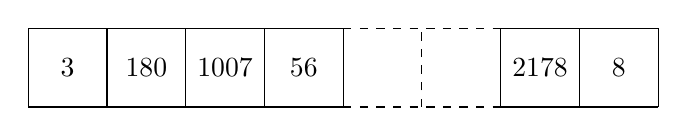
\begin{tikzpicture}
        \draw (0,0)grid(4,1);
        \draw[dashed] (4,0)grid(6,1);
        \draw (6,0)grid(8,1);
        \node at(0.5,0.5){3};
        \node at(1.5,0.5){180};
        \node at(2.5,0.5){1007};
        \node at(3.5,0.5){56};
        \node at(6.5,0.5){2178};
        \node at(7.5,0.5){8};


    \end{tikzpicture}
    \captionof{figure}{Parcours séquentiel}
\end{center}

\end{frame}

\begin{frame}
    \frametitle{}

    \begin{aretenir}[]
        Dans le pire des cas la complexité temporelle de la recherche dépend du nombre d'éléments.
        $$O(n)$$
        \end{aretenir}
\note{cas où l'élément n'est pas présent}
\end{frame}

\begin{frame}
    \frametitle{}

    \begin{activite}
        \begin{enumerate}
            \item Écrire la fonction \textbf{\texttt{recherche\_classique(tab: list, cherche: int) $\rightarrow$ bool}} qui renvoie \textbf{\texttt{True}} si l'entier \textbf{\texttt{cherche}} est présent dans le tableau.
            \item Tester la fonction: vérifier si le nombre 575000 a été choisi par une personne.
            \item À l'aide de la méthode \textbf{\texttt{time}} de la bibliothèque \textbf{\texttt{time}} mesurer la durée d'exécution de la fonction.
        \end{enumerate}
    \end{activite} 

\end{frame}
\begin{frame}
    \frametitle{Correction}

    \lstinputlisting[firstline=13 ,lastline=21, basicstyle=\small , xleftmargin=2em, xrightmargin=2em]{"scripts/dicho.py"}

\end{frame}
\begin{frame}[fragile]
    \frametitle{Correction}

    \lstinputlisting[firstline=41 ,lastline=44 , basicstyle=\small, xleftmargin=2em, xrightmargin=2em]{"scripts/dicho.py"}
\begin{center}
\begin{lstlisting}[language=Bash , basicstyle=\small, xleftmargin=2em, xrightmargin=2em]
False
0.0066792964935302734
\end{lstlisting}
\captionof*{code}{Exemple de résultat}
\end{center}
\end{frame}
\section{Recherche dans un tableau trié}
\subsection{Des données ordonnées}
\begin{frame}
    \frametitle{Des données ordonnées}

    Imaginons maintenant la même expérience mais prenons la peine de trier les éléments au fur et à mesure de leur ajout dans le tableau de données.
\begin{center}
    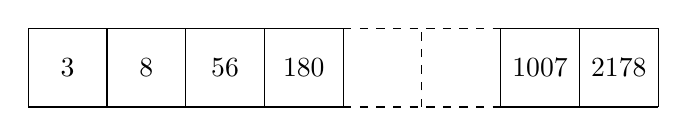
\begin{tikzpicture}
        \draw (0,0)grid(4,1);
        \draw[dashed] (4,0)grid(6,1);
        \draw (6,0)grid(8,1);
        \node at(0.5,0.5){3};
        \node at(1.5,0.5){8};
        \node at(2.5,0.5){56};
        \node at(3.5,0.5){180};
        \node at(6.5,0.5){1007};
        \node at(7.5,0.5){2178};
    \end{tikzpicture}
    \captionof{figure}{Tableau trié}
\end{center}

\end{frame}
\begin{frame}
    \frametitle{}

    \begin{activite}
        Pour simplifier nous allons utiliser la méthode \textbf{\texttt{sort}} pour trier les données.
        \begin{enumerate}
            \item Construire par compréhension un tableau de dix mille entiers compris entre 0 et 1000000.
            \item Trier le tableau.
        \end{enumerate}
        \end{activite}

\end{frame}
\begin{frame}[fragile]
    \frametitle{Correction}

    \begin{center}
    \begin{lstlisting}[language=Python , basicstyle=\small, xleftmargin=2em, xrightmargin=2em]
entiers = [randint(0, 1000000) for _ in range(100000)]
entiers.sort()
\end{lstlisting}
    \captionof*{code}{Jeu de données}
    \label{CODE}
    \end{center}

\end{frame}
\subsection{Recherche dichotomique}
\begin{frame}
    \frametitle{Recherche dichotomique}

    Les données étant triées, le principe de la dichotomie, pour chercher la présence d'un élément, consiste à:
\begin{itemize}
    \item couper le tableau en deux parties égales,
    \item ne garder que la partie contenant l'élément,
    \item répéter l'opération jusqu'à trouver l'élément ou avoir une partie vide.
\end{itemize}
\note{à peu près égales selon parité}
\end{frame}
\begin{frame}
    \frametitle{}

    Cherchons 765 dans le tableau suivant:
\begin{center}
    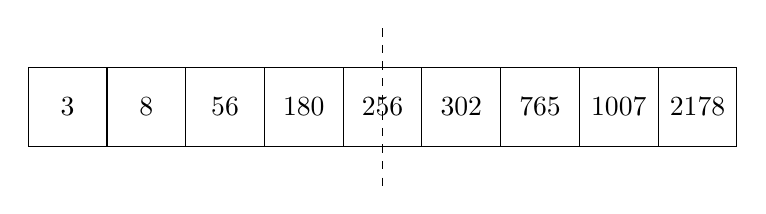
\begin{tikzpicture}
        \draw (0,0)grid(9,1);
        \node at(0.5,0.5){3};
        \node at(1.5,0.5){8};
        \node at(2.5,0.5){56};
        \node at(3.5,0.5){180};
        \node at(4.5,0.5){256};
        \node at(5.5,0.5){302};
        \node at(6.5,0.5){765};
        \node at(7.5,0.5){1007};
        \node at(8.5,0.5){2178};
        \draw[dashed] (4.5,1.5)--(4.5,-0.5);
    \end{tikzpicture}
    \captionof{figure}{Séparons les données en deux parties}
\end{center}

\end{frame}
\begin{frame}
    \frametitle{}

    \begin{center}
        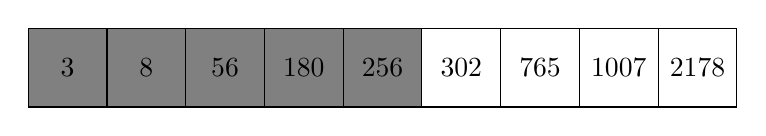
\begin{tikzpicture}
            \fill[gray] (0,0) -- (5,0) -- (5,1) -- (0,1)-- cycle;
            \draw (0,0)grid(9,1);
            \node at(0.5,0.5){3};
            \node at(1.5,0.5){8};
            \node at(2.5,0.5){56};
            \node at(3.5,0.5){180};
            \node at(4.5,0.5){256};
            \node at(5.5,0.5){302};
            \node at(6.5,0.5){765};
            \node at(7.5,0.5){1007};
            \node at(8.5,0.5){2178};
        \end{tikzpicture}
        \captionof{figure}{256 n'est pas le nombre recherché et il est inférieur à 765}
    \end{center} 

\end{frame}
\begin{frame}
    \frametitle{}

    \begin{center}
        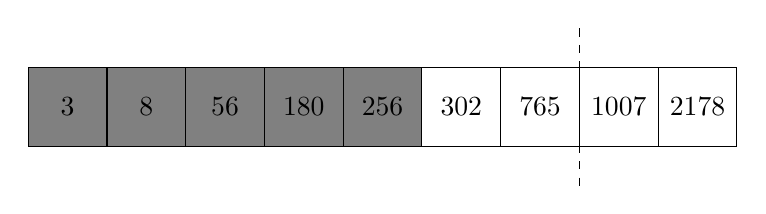
\begin{tikzpicture}
            \fill[gray] (0,0) -- (5,0) -- (5,1) -- (0,1)-- cycle;
            \draw (0,0)grid(9,1);
            \node at(0.5,0.5){3};
            \node at(1.5,0.5){8};
            \node at(2.5,0.5){56};
            \node at(3.5,0.5){180};
            \node at(4.5,0.5){256};
            \node at(5.5,0.5){302};
            \node at(6.5,0.5){765};
            \node at(7.5,0.5){1007};
            \node at(8.5,0.5){2178};
            \draw[dashed] (7,1.5)--(7,-0.5);
        \end{tikzpicture}
        \captionof{figure}{Séparons les données restantes en deux parties}
    \end{center}

\end{frame}
\begin{frame}
    \frametitle{}

    \begin{center}
        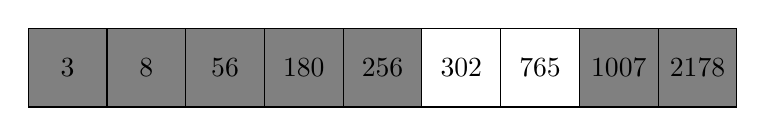
\begin{tikzpicture}
            \fill[gray] (0,0) -- (5,0) -- (5,1) -- (0,1)-- cycle;
            \fill[gray] (7,0) -- (9,0) -- (9,1) -- (7,1)-- cycle;
            \draw (0,0)grid(9,1);
            \node at(0.5,0.5){3};
            \node at(1.5,0.5){8};
            \node at(2.5,0.5){56};
            \node at(3.5,0.5){180};
            \node at(4.5,0.5){256};
            \node at(5.5,0.5){302};
            \node at(6.5,0.5){765};
            \node at(7.5,0.5){1007};
            \node at(8.5,0.5){2178};
        \end{tikzpicture}
        \captionof{figure}{Nous pouvons éliminer la partie supérieure à 765}
    \end{center}

\end{frame}
\begin{frame}
    \frametitle{}

    \begin{center}
        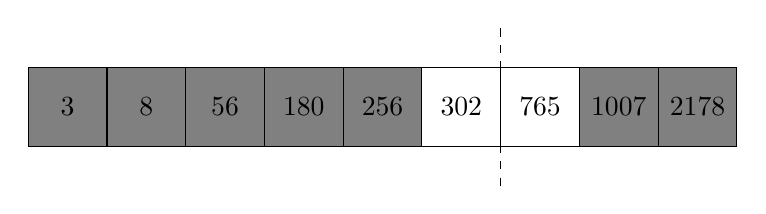
\begin{tikzpicture}
            \fill[gray] (0,0) -- (5,0) -- (5,1) -- (0,1)-- cycle;
            \fill[gray] (7,0) -- (9,0) -- (9,1) -- (7,1)-- cycle;
            \draw (0,0)grid(9,1);
            \node at(0.5,0.5){3};
            \node at(1.5,0.5){8};
            \node at(2.5,0.5){56};
            \node at(3.5,0.5){180};
            \node at(4.5,0.5){256};
            \node at(5.5,0.5){302};
            \node at(6.5,0.5){765};
            \node at(7.5,0.5){1007};
            \node at(8.5,0.5){2178};
            \draw[dashed] (6,1.5)--(6,-0.5);
        \end{tikzpicture}
        \captionof{figure}{Dernière séparation}
    \end{center}

\end{frame}
\begin{frame}
    \frametitle{}

    \begin{center}
        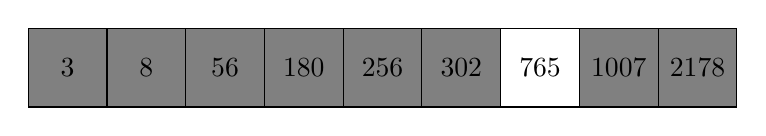
\begin{tikzpicture}
            \fill[gray] (0,0) -- (6,0) -- (6,1) -- (0,1)-- cycle;
            \fill[gray] (7,0) -- (9,0) -- (9,1) -- (7,1)-- cycle;
            \draw (0,0)grid(9,1);
            \node at(0.5,0.5){3};
            \node at(1.5,0.5){8};
            \node at(2.5,0.5){56};
            \node at(3.5,0.5){180};
            \node at(4.5,0.5){256};
            \node at(5.5,0.5){302};
            \node at(6.5,0.5){765};
            \node at(7.5,0.5){1007};
            \node at(8.5,0.5){2178};
        \end{tikzpicture}
        \captionof{figure}{765 a été trouvée en trois itérations}
    \end{center}

\end{frame}
\begin{frame}
    \frametitle{En pratique, on utilise les indices pour trouver le milieu.}

    \begin{center}
        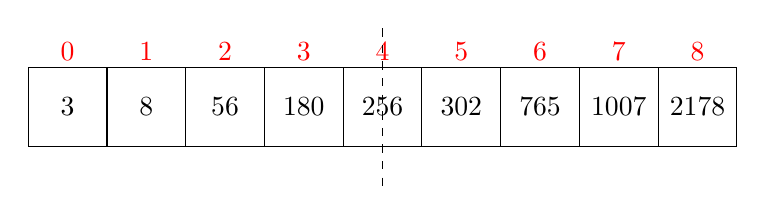
\begin{tikzpicture}
            \draw (0,0)grid(9,1);
            \foreach \a/\b in {0/3, 1/8, 2/56, 3/180, 4/256, 5/302, 6/765, 7/1007, 8/2178}
            {\node at (\a+0.5,0.5) {\b};
            \node[red] at (\a+0.5,1.2) {\a};}
            \draw[dashed] (4.5,1.5)--(4.5,-0.5);
        \end{tikzpicture}
        \captionof{figure}{$\dfrac{8+0}{2}=4$ l'indice médian est 4}
    \end{center}
\begin{itemize}
    \item 256 n'est pas le nombre recherché,
    \item il est inférieur au nombre recherché.
\end{itemize}
\end{frame}
\begin{frame}
    \frametitle{}

    \begin{center}
        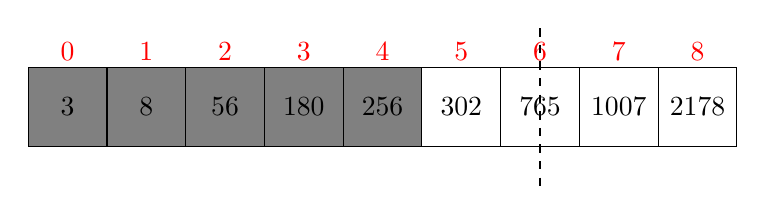
\begin{tikzpicture}
            \fill[gray] (0,0) -- (5,0) -- (5,1) -- (0,1)-- cycle;
            \draw (0,0)grid(9,1);
            \foreach \a/\b in {0/3, 1/8, 2/56, 3/180, 4/256, 5/302, 6/765, 7/1007, 8/2178}
            {\node at (\a+0.5,0.5) {\b};
            \node[red] at (\a+0.5,1.2) {\a};}
            \draw[dashed] (6.5,1.5)--(6.5,-0.5);
        \end{tikzpicture}
        \captionof{figure}{$\dfrac{8+5}{2}=6$ l'indice médian est 6}
    \end{center}
\begin{itemize}
    \item 765 est le nombre recherché,
    \item la recherche s'arrête.
\end{itemize}
\note[item]{l'indice est un entier}
\end{frame}
\begin{frame}
    \frametitle{}

    
    \begin{activite}
        Écrire la fonction \textbf{\texttt{recherche\_dicho(tab: list, cherche: int) $\rightarrow$ bool}} qui applique le principe de la dichotomie. Pour séparer les données en deux parties (à peu près) égales il faudra calculer l'indice médian de la partie encore valide.
        \end{activite}
\end{frame}
\begin{frame}
    \frametitle{Correction}

    \lstinputlisting[firstline=24 ,lastline=26 , basicstyle=\small, xleftmargin=2em, xrightmargin=2em]{"scripts/dicho.py"}

\end{frame}
\begin{frame}
    \frametitle{Correction}

    \lstinputlisting[firstline=27 ,lastline=28 , basicstyle=\small, xleftmargin=2em, xrightmargin=2em]{"scripts/dicho.py"}

\end{frame}
\begin{frame}
    \frametitle{Correction}

    \lstinputlisting[firstline=29 ,lastline=30 , basicstyle=\small, xleftmargin=2em, xrightmargin=2em]{"scripts/dicho.py"}

\end{frame}
\begin{frame}
    \frametitle{Correction}

    \lstinputlisting[firstline=31 ,lastline=34 , basicstyle=\small, xleftmargin=2em, xrightmargin=2em]{"scripts/dicho.py"}

\end{frame}
\begin{frame}
    \frametitle{Correction}

    \lstinputlisting[firstline=24 ,lastline=36 , basicstyle=\small, xleftmargin=2em, xrightmargin=2em]{"scripts/dicho.py"}

\end{frame}
\subsection{Efficacité}
\begin{frame}
    \frametitle{Efficacité}
    À chaque itération la quantité de données (notée \textbf{n}) à étudier est divisée par deux. Dans le pire des cas, on divise jusqu'à ce que la taille de la partie restante soit inférieure ou égale à 1.
\note{0 = pas trouvé}
    {\Large$$\dfrac{n}{2^x}=1$$
    $$\Leftrightarrow n=2^x$$}
    

\end{frame}
\begin{frame}
    \frametitle{}

    \begin{activite}
        \begin{enumerate}
            \item Encadrer la valeur de \emph{x} entre deux entiers, si le tableau contient $n=10000$ éléments.
            \item Mesurer la durée d'exécution de la fonction et la comparer à celle de la recherche classique.
        \end{enumerate}
        \end{activite}

\end{frame}
\begin{frame}
    \frametitle{Correction}

    {\Large $$2^{13}=8192 < x < 2^{14}=16384$$}

\end{frame}

\begin{frame}[fragile]
    \frametitle{Correction}

    \lstinputlisting[firstline=47 ,lastline=50 , basicstyle=\small, xleftmargin=2em, xrightmargin=2em]{"scripts/dicho.py"}
\begin{center}
\begin{lstlisting}[language=Bash , basicstyle=\small, xleftmargin=2em, xrightmargin=2em]
False
0.0009853839874267578
\end{lstlisting}
\captionof*{code}{Exemple de résultat}
\end{center}
\note{facteur 10}
\end{frame}
\begin{frame}
    \frametitle{}

    \begin{aretenir}[]
        La complexité temporelle de la recherche dichotomique est:
        {\Large$$ \log_2{n} =x$$}
        \end{aretenir}
\note{$\log_2 n = \dfrac{\ln n}{\ln 2}$}
\end{frame}
\begin{frame}
    \frametitle{Code complet}

    Le code complet se trouve \href{https://cviroulaud.github.io/premiere/algorithmique/recherche-dichotomique/scripts/dicho.zip}{ici}.

\end{frame}
\end{document}